\chapter{Non-parametric Modeling}
\def\thisDir{ch03-lrm}
\tikzsetfigurename{ch03fig}
\label{sec:nonparametric}
% \myEpigraph{}{}{}

\section{Introduction}
\label{sec:nonparametric:introduction}

Whereas many areas of system identification focus on parametric identification and/or parameter estimation, non-parametric techniques have recently received new research interest from the community.

\begin{itemize}
\item \TODO{explain non-parametric}
\item \TODO{explain why non-parametric is good}
\end{itemize}

The measurement of \glspl{FRF} of dynamic systems is an important step in many technical applications, often used as a simple visualization of the system dynamics.
\gls{FRF} measurement techniques are discussed, for instance, in
\citep{Schoukens1998,Schoukens2006LPM,Guillaume1996,Broersen1995,Pintelon2010LPM1,Antoni2007FRF,Pintelon2012}, and applied to practical devices and systems~\citep{Lim2010,Robinson1990,Behjat2010}, among others.
Besides, \glspl{FRF} have been shown to provide a quick insight into the dynamic properties of \gls{LTI} systems.
This capability is very useful for model validation and/or model selection~\citep{Pintelon2012}.

Estimating a non-parametric \gls{FRF} is often a key step in the analysis and/or design of physical systems.
However, obtaining a good-quality non-parametric \gls{FRF} from a measured input-output data set can prove difficult due to the presence of noise and measurement time limitations to observe lightly-damped dynamics well.

Recently, there has been a renewed interest in the development of non-parametric estimators to estimate the \gls{FRF} of a system.
Many of these approaches have focused on separating the periodic response (i.e. the \gls{FRF}), the measurement noise and leakage contributions of the spectrum by exploiting the structure that those different contributions exhibit.


\citep{Pintelon2010LPM1},\citep{Pintelon2010LPM2},\citep{McKelvey2012LRM}


% \paragraph*{Contributions}
% In this paper, the existing \gls{LRM} is extended to the \gls{LRIC} that does not suffer from  the bias that is present in the \gls{LRM}.
% An extensive study is carried out to compare the performance of the \gls{LPM}, \gls{LRM} and \gls{LRIC} to describe resonant systems under varying conditions of the signal-to-noise ratio.
% Also, a pragmatic model-order-selection tool for the \gls{LPM} and \gls{LRM} is introduced.

\paragraph*{Outline}
\secref{sec:theory} introduces theory of estimating \glspl{FRF} and the relevant local modeling techniques.
In \secref{sec:simulations} the performance of the different modeling methods is investigated by means of simulations.
The methods are then illustrated on measurements of mechanical systems in \secref{sec:measurements}.
Finally, conclusions are presented in \secref{sec:conclusion}.


\begin{itemize}
    \item \TODO{choice $s$ or $z$}
    \item \TODO{bounds RMSE, Bias, StdDev}
    \item \TODO{derivation Bias}
    \item \TODO{comparison LPM/LRM}
      \begin{itemize}
        \item \TODO{Good LPM window}
        \item \TODO{Good LRM window}
      \end{itemize}
    \item \TODO{influence of noise filter: mismatch with model}
    \item \TODO{comparison LRM/LRik (LBTLS)}
\end{itemize}

\section{Local modeling approaches}
\label{sec:theory}

Consider a discrete-time generalized output-error \gls{LTI} set-up, excited by the input signal $u[n]$.
For an infinite data length, such a system can be described in the time domain by
\begin{equation}
  y[n] = \ezbrace{\true{G}(z) u[n]}{\true{y}[n]} + \ezbrace{\true{H}(z) \true{e}[n]}{v[n]} \text{ with } n \in \IntegerNumbers
  \label{eq:output-error-TD-infinite}
\end{equation}
where $v[n]$ is filtered white noise, $v[n] = \true{H}(z) \true{e}[n]$ where $z^{-1}$ is the backward shift operator, i.e. $z^ {-1}x[n] = x[n-1]$.
The transfer functions $\true{G}$ and $\true{H}$ are rational functions that are stable and causal.

During typical measurements, however, $y[n]$ and $u[n]$ are only measured over a limited time span, i.e. $n \in \set{0,1,\ldots,N-1}$.
This introduces transient terms $t_{\bullet}$ in this relationship~\citep{Pintelon1997ARB}:
\begin{equation}
y[n] = \true{G}(z) u[n] + \true{H}(z) \true{e}[n] + \ezbrace{t_G[n] + t_H[n]}{t[n]}
\label{eq:output-error-TD-finite}
\end{equation}
where $t_G[n]$ and $t_H[n]$ are due to the different conditions of respectively $\true{G}$ and $\true{H}$ at the beginning and end of the measurement record~\citep{Pintelon1997ARB}.
Both terms can be lumped together as $t[n]$, which is often~\citep{Pintelon2010LPM1} determined predominantly by $t_G[n]$.

\begin{definition}\label{def:DFT}
The $N$-points \glsfirst{DFT} of a signal $x(n\Ts) = x[n]$ with $n \in \set{0,\ldots,N-1}$ is
\begin{equation}
  X \left[ k \right] =
  X \left( \omega_k \right)
  \isdef
  \frac{1}{\sqrt{N}}\sum_{n=0}^{N-1} x \left( n \Ts \right)  \exponent{- j \omega_k n \Ts }
  \label{eq:DFT}
\end{equation}
where $\omega_k \isdef \tfrac{2 \pi k }{N \Ts}$, $k \in \set{0,\ldots,N-1}$ and $\Ts$ is the sampling time.
\end{definition}

By applying the \gls{DFT}~\eqref{eq:DFT} to both sides of \eqref{eq:output-error-TD-finite}, one obtains its frequency-domain counterpart:
\begin{align}
    Y \left( \omega_k \right) 
    & = \true{G} \left( \omega_k \right) U \left( \omega_k \right) 
      + \true{H} \left( \omega_k \right) E \left( \omega_k \right)
      + T \left( \omega_k \right)\\
      &= \true{G} \left( \omega_k \right) U \left( \omega_k \right)  + V(\omega_k) + T(\omega_k)
      \text{.}
  \label{eq:output-error-FD}
\end{align}

In this paper, we focus on using local modeling to separate the different terms, i.e.
\begin{itemize}
  \item the transfer function $\true{G}$,
  \item the leakage term $T$, and
  \item the noise term $V$.
\end{itemize}

\subsection{Local modeling}
Local modeling methods  exploit the `smoothness' (or conversely `roughness') of the different terms of \eqref{eq:output-error-FD} over the frequency $\omega$.
In particular, we will assume that $U(\omega)$ is `rough' over the frequency~\citep{Schoukens2009LPM}, e.g. as is the case for noise excitations or random phase multisines (see further).
On the other hand, it is well-known that the transfer functions $\true{G}$, $\true{H}$ and hence also the corresponding transient contributions $T = T_G + T_H$ are smooth over the frequency.
As such, these smooth contributions can be approximated well around each frequency $\omega_k$ using a local rational model:
\begin{align}
  \true{G}(\omega_{k}+d) 
  &\approx
  \frac{\sum_{i=0}^{\order{B}} b_i d^i}
            {1 + \sum_{i=1}^{\order{A}} a_i d^i}
    &\isdef
    \frac{\LocalModel[k]{B}(d)}%
           {\LocalModel[k]{A}(d)} 
           = \LocalModel[k]{G}(d)
  \text{,}
  \label{eq:LRM:model:G}
  \\
  \true{T}(\omega_k + d) &\approx
  \frac{\sum_{i=0}^{\order{C}} c_i d^i}
            {1 + \sum_{i=1}^{\order{A}} a_i d^i}
    &\isdef 
      \frac{\LocalModel[k]{C}(d)}%
           {\LocalModel[k]{A}(d)}
      = \LocalModel[k]{T}(d)
  \text{.}
  \label{eq:LRM:model:T}
\end{align}

In these expressions, we denote $\LocalModel[k]{G}$ and $\LocalModel[k]{T}$ for the local model for respectively transfer function and the transient.
Note that such local quantities (which depend on the frequency bin $k$) are denoted in bold throughout this paper.
To alleviate the notations, the subscript $k$ is often omitted.

To estimate the local parameters $\LocalVector{\theta} = \mat{a_1\; \cdots\; b_0 \cdots\; c_0\; \cdots}^{\T}$ in \eqref{eq:LRM:model:G} and \eqref{eq:LRM:model:T}, we consider a local window
\begin{equation}
  \LocalWindow[k] 
  \isdef
  \Set{
    \omega_{k+r} 
    | 
    r \in \LocalShifts{k}
  }
\end{equation}
with $\LocalShifts{k} \isdef \Set{-\numel{W}, -\numel{W}+1, \ldots, 0, \ldots, \numel{W}}$
such that the local window around $\omega_k$ consists of $\numel{\LocalWindow} = 2 \numel{W} + 1$ bins. 
If one denotes the input/output spectra in such a local frequency window $\LocalWindow[k]$ as
\begin{equation}
  \LocalVector{U}_k \isdef 
  \mat{
    U(\omega_{k-N_W})\\
    \vdots\\
    U(\omega_{k})\\
    \vdots\\
    U(\omega_{k+N_W})\\
  }
  \text{ and }
  \LocalVector{Y}_k \isdef 
  \mat{
    Y(\omega_{k-N_W})\\
    \vdots\\
    Y(\omega_{k})\\
    \vdots\\
    Y(\omega_{k+N_W})\\
  }
  \text{,}
\end{equation}
and similarly for the other quantities, equation \eqref{eq:output-error-FD} limited to $\LocalWindow[k]$ can be written as
$
  \LocalVector{Y}_k  = {\true{\LocalVector{G}}}_k \hadamard \LocalVector{U}_k + \LocalVector{T}_k + \LocalVector{V}_k
$, where $\hadamard$ denotes the entry-wise product (or Hadamard product).
Substituting $\true{\LocalVector{G}}$ and $\LocalVector{T}$ with the local models $\LocalModel{G}$ and $\LocalModel{T}$ and neglecting the influence of $\LocalVector{V}$ yields
\begin{equation}
  \LocalVector{Y} 
  \approx 
  \hat{\LocalVector{Y}} 
    =
      \LocalModel{G} \hadamard \LocalVector{U} + \LocalModel{T}
      \text{.}
      \label{eq:local-system-equations}
\end{equation}
Note that this encompasses $\numel{\Window}$ complex equations in the $\numel{\theta} = \numel{A} + \numel{B} + \numel{C} + 2$  unknown complex model parameters ($a_i$, $b_i$ and $c_i$ in \eqref{eq:LRM:model:G} and \eqref{eq:LRM:model:T}).
Consequently, a necessary condition to compute the model parameters is that
\begin{equation}
  \DOF = \numel{\Window} - \numel{\theta}
       = 2 \numel{W} - \numel{A} - \numel{B} - \numel{C} - 1
\end{equation}
is positive.
To effectively compute the local model parameters, the equation error in \eqref{eq:local-system-equations} is minimized by formulating a quadratic cost function:
\begin{equation}
  \LocalVector{\CostFunc{\LRIC}} 
    \isdef 
      \left( \LocalVector{Y}  -  \LocalModel{G} \hadamard \LocalVector{U} - \LocalModel{T} \right)^{\HT} 
      \left( \LocalVector{Y}  -  \LocalModel{G} \hadamard \LocalVector{U} - \LocalModel{T} \right)
   \label{eq:costfunc:LRIC}
   \text{.}
\end{equation}
Due to the presence of the denominator of $\LocalModel{G} = \frac{\LocalModel{B}}{\LocalModel{A}}$, the equation error is not linear in the parameters $a_i$ and hence \eqref{eq:costfunc:LRIC} requires time-consuming iterative optimization schemes to obtain a parameter estimate.

\subsection{The Local Rational Method}
The \gls{LRM} as first introduced by \citep{McKelvey2012LRM}, overcomes the computational burden of an iterative procedure by weighting the equation error by the denominator polynomial $\LocalModel{A}$  akin to the procedure in \citep{Levy1959}.
I.e. the \gls{LRM} procedure tries to minimize the equation error in
\begin{equation}
  \LocalModel{A}\LocalVector{Y} \approx \LocalModel{B} \LocalVector{U}  - \LocalVector{C}
  \text{,}
\end{equation}
for which the corresponding cost function is
\begin{equation}
  \LocalVector{\CostFunc{\LRM}}
  \isdef 
  \left( \LocalModel{A} \hadamard \LocalVector{Y}  -  \LocalModel{B} \hadamard \LocalVector{U} - \LocalModel{C} \right)^{\HT} 
      \left( \LocalModel{A} \hadamard \LocalVector{Y}  -  \LocalModel{B} \hadamard \LocalVector{U} - \LocalModel{C} \right)
      \text{.}
\end{equation}
Here, $A\hadamard B$ denotes the Hadamard, or element-wise, product of matrices $A$ and $B$ which have identical dimensions.
In \MATLAB the corresponding operator is \mcode{.*}.
Equivalently, the last equation can be rewritten as a linear regression problem
\begin{equation}
  \LocalVector{Y} = \LocalVector{K} \LocalVector{\theta} + \LocalModel{V}
\end{equation}
where $\LocalVector{K}$ is the so-called design matrix (or observation matrix):
\begin{align}
  \label{eq:nparam:designMatrix}
  \LocalVector{K} 
    & \isdef 
  \mat{
     \LocalVector{K}_A &
     \LocalVector{K}_B & 
     \LocalVector{K}_C
  }\\
  \LocalVector{K}_A 
    &\isdef
    \mat{
      \LocalVector{Y} \hadamard \LocalVector{d}^1 &
      \cdots &
      \LocalVector{Y} \hadamard \LocalVector{d}^{\numel{A}}
    }\\
  \LocalVector{K}_B 
    &\isdef
    \mat{
      \LocalVector{U} \hadamard \LocalVector{d}^0 &
      \cdots &
      \LocalVector{U} \hadamard \LocalVector{d}^{\numel{B}}
    }\\
  \LocalVector{K}_C
    &\isdef
    \mat{
      \LocalVector{d}^0 &
      \cdots &
      \LocalVector{d}^{\numel{C}}
    }\\
    \LocalVector{d}^{n} & \isdef
    \mat{
      (-\numel{W})^{n} &
      \cdots &
      (\numel{W})^{n}
    }^{\T}
    \text{ with $n \in \mathbb{Z}$.}
\end{align}
and $\LocalModel{V}$ are the model residuals.
This formulation facilitates to solve the problem in a one-step approach:
\begin{equation}
  \LocalVector{\theta}_{\LRM} 
    \isdef \pinv{\LocalVector{K}} \LocalVector{Y}
    = \left( \LocalVector{K}^{\HT} \LocalVector{K} \right)^{-1} \LocalVector{K}^{\HT} \LocalVector{Y}
\end{equation}
where $\pinv{K}$ denotes the Moore-Penroose pseudo-inverse of $K$.

\TODO{hier voortschrijven}

\subsection{The Local Rational Method with Iterative Cost}

\subsection{Notes}

Since it is well-known that the Vandemonde structure in the design matrix \eqref{eq:nparam:designMatrix} leads to numerical ill-conditioning for higher model complexities, additional measures are taken to improve numerical conditioning.
To improve numerical conditioning~\citep{Pintelon2005} of the estimation problem, we substitute $d = \dw{r}{k}$ in equations \eqref{eq:LRM:model:G} and \eqref{eq:LRM:model:T}
\begin{equation}
\dw{r}{k} \isdef \frac{\omega_{k+r} - \omega_k}{\Delta \omega_k}
\label{eq:freqScaling}
\end{equation}
where
\begin{equation}
  \Delta \omega_k \isdef
  \max
  \Set{
    \abs{ \omega_k - \omega_j} |  \vphantom{\frac{a}{b}}  \omega_j \in \LocalWindow[k]
  }
\end{equation}
such that $\abs{\dw{r}{k}} \leq 1$ when $r \in \LocalShifts{k}$.

\TODO{define local cost}
\TODO{define local design matrix}


\section{Theory: bias}
\label{sec:biascalc}
Since the local design matrix \eqref{eq:nparam:designMatrix} contains the noisy output spectrum $\LocalVector{Y}$ when $\numel{A} > 0$, the \gls{LRM} is expected to be a biased estimator.
In this section, we will derive expressions for the bias such that it can be quantified how important this bias is in different situations.

To determine the bias, an approach similar to \citep[Appendix A]{Guillaume1995} is followed.
Let us denote the expected value of the cost function over all measurements $\LocalVector{Z}$ as
\begin{align}
  \ELSCost{\theta}
              & \isdef 
                   \E[\LocalVector{Z}]%
                         {    
                                \LSCost{\LocalVector{\theta}, \LocalVector{Z}}} \\
              & = \ELSCost[0]{\theta} + \ELSCost[n]{\theta} \\
    \ELSCost[0]{\theta} & \isdef 
            \frac{1}{F} 
                \sum_{r} 
                     \left| 
                             \LocalModel{A}(r, \LocalVector{\theta}) \true{\LocalVector{Y}}
                          - \LocalModel{B}(r, \LocalVector{\theta}) \true{\LocalVector{U}}
                          - \LocalModel{C}(r, \LocalVector{\theta}) 
                    \right|^2 \\
    \ELSCost[n]{\theta} & \isdef 
              \frac{1}{F} 
                     \sum_{r} 
                              \left| \LocalModel{A}(r,\LocalVector{\theta}) \right|^2 
                              \sigma_V^2
\end{align}
where $\true{\LocalVector{U}}$ and $\true{\LocalVector{Y}}$ denote the `true' (noiseless) input-output spectra in the local window.
Note that this function is a quadratic function of $\LocalVector{\theta}$ and hence it can be represented exactly by its second order Taylor series around $\true\theta$:
\begin{multline}
  \ELSCost{\theta} = \ELSCost{\true\theta} 
  + \PartialDerivative{\ELSCost{\true\theta}}{\true\theta}  \left( \theta - \true\theta \right) %\\
  + \frac{1}{2} \left( \theta - \true\theta \right)^{\T} 
  \PartialDerivative[2]{\ELSCost{\true\theta}}{\true\theta} 
   \left( \theta - \true\theta \right)
   \text{.}
\end{multline}
The minimizer $\estimated\theta$ of this function can be obtained by equating the derivative
\begin{equation}
  \PartialDerivative{\ELSCost{\estimated\theta}}
                                          {\estimated\theta} 
  = 
  \left( \PartialDerivative{\ELSCost{\true\theta}}{\true\theta} \right)^{\T} 
  + \PartialDerivative[2]{\ELSCost{\true\theta}}{\true\theta} \left( \estimated\theta - \true\theta \right)
\end{equation}
to zero.
This is equivalent to 
\begin{equation}
  \left( \estimated\theta - \true\theta \right) 
  = 
  - \left(   \PartialDerivative[2]{\ELSCost{\true\theta}}{\true\theta} \right)^{-1}  
     \left( \PartialDerivative{\ELSCost{\true\theta}}{\true\theta} \right)^{\T}
  \text{.}
\end{equation}
which expresses the bias $\Delta\theta = \left( \estimated\theta - \true\theta \right)$ of the estimated parameters.
Remark that 
\begin{equation}
  \PartialDerivative{\ELSCost{\true\theta}}{\true\theta}  
  = 
  \PartialDerivative{\ELSCost[0]{\theta} + \ELSCost[n]{\theta} }{\true\theta} 
  = 
  \PartialDerivative{\ELSCost[n]{\theta} }{\true\theta} 
\end{equation}
since $\ELSCost[0]{\theta}$ is minimized in $\true\theta$ by definition.
As such, the bias on the parameters can be simplified to
\begin{equation}
  \Delta\theta = 
  - \left(   \PartialDerivative[2]{\ELSCost{\true\theta}}{\true\theta^2} \right)^{-1} 
     \left( \PartialDerivative{\ELSCost[n]{\true\theta}}{\true\theta} \right)^{\T}
  \text{.}
  \label{eq:nparam:bias-basic}
\end{equation}

Do note that the estimated parameters $\theta \in \ComplexMatrix{\nth \times 1}$ but that $\ELSCost{\theta}$ is a real-valued function.
In contrast to a complex-valued function, this requires additional attention when the derivatives are calculated~\citep{Messerschmitt2006} and~\citep[Section 15.9]{Pintelon2012} since $\ELSCost{\theta}$ is not an analytic function.
Particularly, the function $\ELSCost{\theta}$ is regarded as a two-dimensional function $\ELSCost{\theta,\conj{\theta}}$ where $\conj{\theta}$ and $\theta$ are considered as independent variables~\citep{Hjorungnes2007,Hjorungnes2011}.
The derivatives are then computed with respect to these variables.
% Let us introduce the notations
% \begin{equation}
%   \ReIm{X} 
%   \isdef 
%   \begin{bmatrix}
%     \real{X}\\
%     \imag{X}
%   \end{bmatrix}
%   \quad  \text{,} \quad
%   \ReImImRe{X} 
%   \isdef 
%   \begin{bmatrix}
%     \real{X} & -\imag{X}\\
%     \imag{X} & \hphantom{-} \real{X}
%   \end{bmatrix}
% \end{equation}
% and the shorthand $\ReIm{\theta} = \ReImTheta$.
% E.g. in \citet[Section 15.9]{Pintelon2012} and \citet[Section 5.1]{Seber2007}, it is stated that $\ReImImRe{X}$ is isomorphic with $X$ such that operations on a complex matrix $X$ can be written as equivalent operations on the real matrix $\ReImImRe{X}$.
% As a result,
% \begin{align}
%   \Delta\theta &=
%   \left( \mat{1 & j} \kron \Identity{\nth[]}  \right) 
%   \ReIm{\Delta\theta}
%   \\
%   \ReIm{\Delta\theta} &= 
%   - \ReImImRe{ \left(   \PartialDerivative[2]{\ELSCost{\true\theta}}{\true\theta^2} \right)^{-1} }
%     \ReIm{ \left( \PartialDerivative{\ELSCost[n]{\true\theta}}{\true\theta} \right)^{\T}}
% \end{align}
% where $\kron$ denotes the Kronecker product~\citep{Brewer1978}.
To facilitate the derivations, we rewrite the expected value of the cost function in terms of $\theta$ and $\conj{\theta}$:
\begin{align}
   \ELSCost[0]{\theta,\conj{\theta}} & =
      \frac{1}{F}
           \sum_{r}
           \LocalModel{Q}(      r,        \LocalVector{\theta},  \true{      \LocalVector{Y}},  \true{      \LocalVector{U} })
           \LocalModel{Q}(\conj{r}, \conj{\LocalVector{\theta}}, \true{\conj{\LocalVector{Y}}}, \true{\conj{\LocalVector{U}}})
   \\
   \LocalModel{Q}(r, \LocalVector{\theta},  \true{\LocalVector{Y}},  \true{ \LocalVector{U} }) & \isdef
                 \LocalModel{A}(r, \LocalVector{\theta}) \true{\LocalVector{Y}}(r)
               - \LocalModel{B}(r, \LocalVector{\theta}) \true{\LocalVector{U}}(r)
               - \LocalModel{C}(r, \LocalVector{\theta})
    \\             
    \ELSCost[n]{\theta,\conj{\theta}} & =
              \frac{\sigma_V^2}{F} 
                     \sum_{r} 
                               \LocalModel{A}(      r,        \LocalVector{\theta} ) 
                               \LocalModel{A}(\conj{r}, \conj{\LocalVector{\theta}}) 
\end{align}
since $\conj{ \LocalModel{A}(r,\theta)} =  \LocalModel{A}(\conj{r},\conj{\theta}) $, and similar for $\LocalModel{B}$ and $\LocalModel{C}$ and $\LocalModel{Q}$.
Remember also that $\theta = \mat{\theta_A^{\TT} & \theta_B^{\TT} & \theta_C^{\TT}}$.

\paragraph{Contributions to the first order derivative}
The last term in \eqref{eq:nparam:bias-basic}, i.e. the first order derivative,  is given by
\begin{equation}
  \PartialDerivative{\ELSCost[0]{\true\theta, \conj{\true\theta}}}{\theta}
  = 
  \begin{bmatrix}
  \PartialDerivative{\ELSCost[0]{\true\theta, \conj{\true\theta}}}{\theta_A} &
  \PartialDerivative{\ELSCost[0]{\true\theta, \conj{\true\theta}}}{\theta_B} &
  \PartialDerivative{\ELSCost[0]{\true\theta, \conj{\true\theta}}}{\theta_C} &
  \end{bmatrix}
\end{equation}
and split into the parts pertaining to respectively $\LocalModel{A}$, $\LocalModel{B}$ and, $\LocalModel{C}$.
The respective components are given by:
\begin{align}
  \PartialDerivative{\ELSCost[n]{\theta,\conj{\theta}}}{a_i} 
     &= 
     \frac{\sigma_V^2}{F}
     \sum_r r^i \LocalModel{A}(\conj{r},\conj{\LocalVector{\theta}}) 
     & \forall i \in \set{1,\ldots,\order{A}}
     \\
   \PartialDerivative{\ELSCost[n]{\theta,\conj{\theta}}}{b_i} 
   &= 0
   & \forall i \in \set{0,\ldots,\order{B}}
   \\
   \PartialDerivative{\ELSCost[n]{\theta,\conj{\theta}}}{c_i} 
   &= 0
   &\forall i \in \set{0,\ldots,\order{C}}
   \text{.}
\end{align}
It can be seen that only the factors pertaining to $\LocalModel{A}$ are present.
As this term occurs linearly in expression \eqref{eq:nparam:bias-basic}, only $\theta_A$ can incur a bias.
Consequently, only the poles are shifted by the presence of noise.

\TODO{write out subexpressions}
As a first order approximation, the bias on the \gls{FRF} can be written as
\begin{equation}
  \Delta \LocalModel{G}(\omega) 
     \approx 
        \PartialDerivative{\LocalModel{G}(\theta, \omega)}
                                          {\theta} 
      \Delta \theta
      \text{.}
\end{equation}
The derivative in that expression can be evaluated easily
\begin{align}
    \PartialDerivative{\LocalModel{G}(\theta, r)}{\theta} 
     &=
     \begin{bmatrix}
       \PartialDerivative{\LocalModel{G}(\theta,r)}{\theta_A} &
       \PartialDerivative{\LocalModel{G}(\theta,r)}{\theta_B} &
       \PartialDerivative{\LocalModel{G}(\theta,r)}{\theta_C} 
     \end{bmatrix}
     \\
     \PartialDerivative{\LocalModel{G}(\theta, r)}{\theta_A} 
     &=
     \begin{bmatrix}
         r^1 & r^2 & \deemph{\cdots} & r^{\order{A}}
     \end{bmatrix}
     \\
     \PartialDerivative{\LocalModel{G}(\theta, r)}{\theta_B} 
     &=
     \begin{bmatrix}
         1 & r^1 & r^2 & \deemph{\cdots} & r^{\order{B}}
     \end{bmatrix}
     \\
     \PartialDerivative{\LocalModel{G}(\theta, r)}{\theta_C} 
     &=
     \Zero{1 \times \order{C}+1}
     \text{.}
\end{align}

However, the sparsity of $\Delta\theta$ can be exploited such that the bias on the \gls{FRF} is expressed as:
\begin{equation}
  \Delta \LocalModel{G}(\theta,r)
  \approx
  - \LocalModel{A}(r,\theta)^{-2}
\end{equation}

\section{Order selection}
Selecting suitable values of $\nWind$, $\order{B}$, $\order{A}$ and $\order{C}$ obviously affects the quality of the obtained local models.
For local rational models, there are a few insights from parametric system identification that can be retained to make these choices easier.
In particular~\citep{Pintelon2010LPM1}:
\begin{equation}
\order{C} \leq \max\set{\order{B},\order{A}}
\end{equation}
 and from statistical point of view~\citep{Mahata2006}, the degrees of freedom should remain positive such that 
 \begin{equation}
 \nWind \geq \order{B} + \order{A} + \order{C} + 2
 \text{.}
 \end{equation}
 
Different heuristics exist to select the local bandwidth $\nWind$, e.g.~\citet{Fan1995,Thummala2012LPMBW,Stenman2000ASETFE} in the framework of local modeling approaches.
As such, we focus mainly on the selection of the model order hyper-parameters ($\order{A}$, $\order{B}$ and $\order{C}$) for a fixed value of $\nWind$.

Here, we take an approach that decides amongst a group of candidate models $\Set{M_1, \ldots, M_N}$, which model $M_i$ is the best model according to some criterion: i.e. one that captures that system dynamics but remains parsimonious.
To do so, one needs to define a criterion that both takes `goodness-of-fit' (e.g. value of the cost function, $R^2$, \ldots) and model complexity into account to ensure that the model captures only the systematic behavior and not random variations of the particular measurement.
The latter is often done using `cross-validation'.

In statistical learning, many relevant cross-validation approaches exist.
Within the system identification community a few simple approaches have been widely adopted~\citep[Chapter 11]{Pintelon2012} to ensure that one does not overmodel the data.
In the following, a short overview is given of different approaches.

\paragraph{Plug-in methods}
In plug-in methods, a goodness-of-fit criterion (e.g. the log-likelihood function $\LogLikelihood$ of the estimated model $M$ given the estimation dataset $Z$), is penalized with a term accounting for the complexity of the model~\citep{Burnham2002}.
E.g. a common choice is the \gls{AIC}~\citep{Akaike1974} or the \gls{AICc}~\citep{Hurvich1989}, which are defined as
\begin{align}
L_{\mathrm{\AIC}} &=
 - 2  \loglikelihood{M | Z} 
 + 2 \numel{\theta}\\
L_{\mathrm{\AICc}} &= 
- 2  \loglikelihood{M | Z} 
+   \frac{2 \nth\nWind}{\nWind - \nth - 1}
\end{align}
where $\nth$ is the number of  estimated parameters in the model $M(\theta)$.
In the context of local modeling, the \gls{AIC} is a poor choice since it relies on asymptotic arguments of the data set, i.e. $\nWind \to \infty$, which is obviously an unwarranted choice in this context.
The best model among a set of $q$ possible models $\Set{M_1, \ldots, M_q}$ is then
\begin{equation}
  M_{\star} \isdef 
  \arg_{M} \min 
  \Set{
    L_{\mathrm{AIC(c)}}(M)
  }
\end{equation}
To select the best model $M_{\star}$ with such a criterion, the model $M_k$ among a set of models $\set{M_1, M_2, \ldots}$ that produces the smallest value of $L_{\mathrm{AICc}}$ is retained.

\begin{remark}
It should be noted that due to $\loglikelihood{M | Z}$ , the value of $L_{\mathrm{AIC(c)}}(M,Z)$ is inherently coupled with the particular dataset $Z$.
Practically, this means that such criteria can only be used to compare local models that are estimated from the same local dataset (i.e. they have the same $\nWind$ and center frequency).
Consequently, the \gls{AICc} criterion cannot be used to select a proper $\nWind$.
\end{remark}

\paragraph{Holdout method}
The so-called `holdout' cross-validation method ensures a good model by first splitting the dataset into two smaller disjoint datasets: e.g. $70\%$ of the data  is used to estimate the model and a goodness-of-fit criterion (e.g. cost function) is used on the remaining data to determine which model has the best out-of-sample performance.
By using independent datasets and assessing the performance of the model on (unseen) validation data, overfitted models can be rejected.

\begin{remark}
Unfortunately, these typical approaches either assume that an abundantly large dataset is available or  assume the models are estimated on  a fixed dataset.
As such, these methods are not ideal for local modeling where the (local) dataset is rather small by design and could change by means of the local bandwidth $N_W$.
\end{remark}

\paragraph{Leave-out cross-validation}
Instead, we use a better-suited cross-validation approach known as \gls{LOOCV} that is related to the \gls{AIC}~\citep{Stone1977}.
Plainly, \gls{LOOCV} cross-validates the model by in turn leaving out each data point, estimating the local model parameters and observing the difference between the omitted data point and the estimate.
In effect, such an approach calculates the \gls{PRESS} for each local model:
\begin{equation}
 \PRESS = 
 \frac{1}{\nWind} 
  \sum_{r \in \LocalShifts{}}
    \abs{\ignoring{r}{\LocalVector{E}}}^2
    \text{,}
\label{eq:PRESS-general}
\end{equation}
where $\ignoring{r}{\LocalVector{E}} = \LocalVector{Y}_{r} - \ignoring{r}{\LocalVector{\estimated{Y}}}$, i.e. the difference between the observed (local) output spectrum at the $r^{\text{th}}$ line and the predicted output spectrum at the same line when the corresponding data point is removed from the estimation procedure.
To select the best model from a set of candidate models, only the model with the lowest \gls{PRESS} value is retained.
In general, this means that \gls{LOOCV} requires estimating $\nWind$ additional models (one for each omitted data point) and hence can be very time-consuming.

For linear models (i.e. $\LocalVector{Y} = \LocalVector{K} \LocalVector{\theta}$, such as for the \gls{LRM} and \gls{LPM}), however, the \gls{PRESS} can be calculated in a single step without estimating any additional models~\citep[Sec.~12.3.2]{Seber2003}:
\begin{equation}
\PRESS = \frac{\LocalVector{E}^{\HT} \LocalVector{W}^{-1} \LocalVector{E}}{2N_W + 1}
\end{equation}
where $\LocalVector{E}$ is the residual vector of the full estimation and $\LocalVector{W}$ is a diagonal weighting matrix with $\LocalVector{W}_{ii} = (1 - \LocalVector{H}_{ii})^{\HT} (1 - \LocalVector{H}_{ii})$ and
$\LocalVector{H} = \LocalVector{K} \pinv{\LocalVector{K}}$ is the so-called `hat-matrix' that is known to be idempotent.

\section{Simulation}
\label{sec:simulations}

In the simulations, we consider a discrete-time second order system with transfer function
\begin{equation}
\true{G}(z) = \frac{0.64587 z + 0.64143}
                                      {47.9426 z^2 - 51.2955 z + 46.9933}
\end{equation}


\begin{figure}
 \centering
  \begin{tikzpicture}[scale=1,>=stealth]
    \matrix[ampersand replacement=\&, row sep=0.3cm, column sep=0.4cm] {
%% FIRST ROW
        \node (E) {$\true{E}$}; \&
        \node[block] (H0) {$\true{H}'$}; \&
        \node[amplifier] (K) {$\kappa$}; \&
        \node[none] (v) {};\\
%% SECOND ROW
        \node[input] (U) {$U$}; \&
        \node[block] (G0) {$\true{G}$}; \&
        \&
        \node[sum]    (sum)  {}; \& 
        \node (Y) {$Y$};\\
    };
    \draw [connector] (E)   -- (H0);
    \draw [connector] (U)   -- (G0);
    \draw [connector] (G0)  -- node[above] {$\true{Y}$} (sum);
    \draw [connector] (H0)  -- (K);
    \draw [connector] (K) -| node[above] {$V$} (sum);
    \draw [connector] (sum) -- (Y);
    % \draw [connector] (y)    -- ++(0,-1.5em) -| node[left,very near end,name=min] {{$-$}} (sum2);

    \begin{pgfonlayer}{background}
      \node[groupbox=black, inner sep=5pt,fit=(H0) (K)] (H0act) {};
      \node at (H0act.north) [color=black, above] {$\true{H}$};
   \end{pgfonlayer}
\end{tikzpicture}

  \caption{Block schematic used in the simulations}
\end{figure}

\TODO{H0}    

\TODO{SNR}
The \gls{SNR} in the system bandwidth $\BW$ is defined as
\begin{equation}
  \SNR_{\BW} \isdef
  \frac{\int_{\BW} \abs{Y_0(\omega)}^2 \dd{\omega}}
            {\int_{\BW} \abs{V(\omega)}^2 \dd{\omega}}
\end{equation}
where $\BW$ is the frequency range of the $3 \unit{dB}$ bandwidth of the system, i.e. where $\abs{G_0} \geq \norm[\infty]{\true G} - 3 \unit{dB}$.

\TODO{plot example spectrums}

We then compute basic statistics of the estimated \glspl{FRF} over all  Monte Carlo runs.
Specifically, the mean value
\begin{align}
  \sampleMean{\bullet}(\omega_k) & 
  \isdef
    \frac{1}{\nMC}
    \sum_{i=1}^{\nMC}
    \atSimulation[i]{\model{\bullet}(\omega_k)}
  &
  \approx
  \expectedValue{\model{\bullet}(\omega_k)}
  \\
  \sampleBias{\bullet}(\omega_k) &
    \isdef
    \frac{1}{\nMC}
    \sum_{i=1}^{\nMC}
    \atSimulation[i]{\model{\bullet}(\omega_k)} - \true{G}(\omega_k)
    &
    \approx
    \Bias{\model{\bullet}(\omega_k)}
    \\
    \sampleVariance{\bullet}(\omega_k) &
    \isdef
    \frac{1}{\nMC - 1}
    \sum_{i=1}^{\nMC}
    \left(\atSimulation[i]{\model{\bullet}(\omega_k)} - \true{G}(\omega_k) \right)
    \conj { \left(\atSimulation[i]{\model{\bullet}(\omega_k)} - \true{G}(\omega_k) \right) }
    &
    \approx
    \Var{\model{\bullet}(\omega_k)}
\end{align}

  % \subsection{Implications of the model structure}
  \subsection{Implications of the noise level}
  % \subsection{Implications of the noise coloring}

\TODO{insert figure: Y(Y,E,T) vs freq}
\TODO{insert figure: err vs SNR}
\paragraph{Noiseless case}
In the noiseless case, one can observe the approximation error that is made by using the \gls{LRM}, \gls{LPM} and \gls{ETFE}.
For the \gls{ETFE}, it can be seen that the error is very high.
This can be expected since the \gls{ETFE} does not separate transient and leakage contributions.
this error only disappears very slowly by measuring a longer record due to the presence of the leakage term.
As such, 
\TODO{figure: RMS, bias, std voor inf SNR}

\TODO{figure: RMS, bias, std voor high SNR}
\TODO{figure: RMS, bias, std voor 20 dB SNR}
\TODO{figure: RMS, bias, std voor 10 dB SNR}

  \section{Measurements}
  \label{sec:measurements}
   \subsection{AVIS}
   % \subsection{F16}

  \section{Conclusion}
  \label{sec:conclusion}

  \begin{itemize}
    \item LRM: extension to LRIC
    \item LRM: derivation of bias
    \item LRM vs LPM: at which settings is LRM better than LPM
    \item LRIC: much slower, performance is somewhat better, but at the cost of a lot of computational power and much harder model selection
    \item practical advice: use LRM rather than LPM unless in very noisy conditions (10 dB), only use LRIC as last resort
  \end{itemize}



\section{Trading off the bias and variance}

\subsection{Order selection}
Selecting suitable values of $\nWind$, $\order{B}$, $\order{A}$ and $\order{C}$ obviously affects the quality of the obtained local models.
For local rational models, there are a few insights from parametric system identification that can be retained to make these choices easier.
In particular~\citep{Pintelon2010LPM1}:
\begin{equation}
\order{C} \leq \max\set{\order{B},\order{A}}
\end{equation}
 and from statistical point of view~\citep{Mahata2006}, the degrees of freedom should remain positive such that 
 \begin{equation}
 \nWind \geq \order{B} + \order{A} + \order{C} + 2
 \text{.}
 \end{equation}
 
Different heuristics exist to select the local bandwidth $\nWind$, e.g.~\citet{Fan1995,Thummala2012LPMBW,Stenman2000ASETFE} in the framework of local modeling approaches.
As such, we focus mainly on the selection of the model order hyper-parameters ($\order{A}$, $\order{B}$ and $\order{C}$) for a fixed value of $\nWind$.

Here, we take an approach that decides amongst a group of candidate models $\Set{M_1, \ldots, M_N}$, which model $M_i$ is the best model according to some criterion: i.e. one that captures that system dynamics but remains parsimonious.
To do so, one needs to define a criterion that both takes `goodness-of-fit' (e.g. value of the cost function, $R^2$, \ldots) and model complexity into account to ensure that the model captures only the systematic behavior and not random variations of the particular measurement.
The latter is often done using `cross-validation'.

In statistical learning, many relevant cross-validation approaches exist.
Within the system identification community a few simple approaches have been widely adopted~\citep[Chapter 11]{Pintelon2012} to ensure that one does not overmodel the data.
In the following, a short overview is given of different approaches.

\paragraph{Plug-in methods}
In plug-in methods, a goodness-of-fit criterion (e.g. the log-likelihood function $\LogLikelihood$ of the estimated model $M$ given the estimation dataset $Z$), is penalized with a term accounting for the complexity of the model~\citep{Burnham2002}.
E.g. a common choice is the \gls{AIC}~\citep{Akaike1974} or the \gls{AICc}~\citep{Hurvich1989}, which are defined as
\begin{align}
L_{\mathrm{\AIC}} &=
 - 2  \loglikelihood{M | Z} 
 + 2 \nth\\
L_{\mathrm{\AICc}} &= 
- 2  \loglikelihood{M | Z} 
+   \frac{2 \nth\nWind}{\nWind - \nth - 1}
\end{align}
where $\nth$ is the number of  estimated parameters in the model $M(\theta)$.
In the context of local modeling, the \gls{AIC} is a poor choice since it relies on asymptotic arguments of the data set, i.e. $\nWind \to \infty$, which is obviously an unwarranted choice in this context.
The best model among a set of $q$ possible models $\Set{M_1, \ldots, M_q}$ is then
\begin{equation}
  M_{\star} \isdef 
  \arg_{M} \min 
  \Set{
    L_{\mathrm{AIC(c)}}(M)
  }
  \text{,}
\end{equation}
which is the only model that is hence retained.

\begin{remark}
It should be noted that due to $\loglikelihood{M | Z}$ , the value of $L_{\mathrm{AIC(c)}}(M,Z)$ is inherently coupled with the particular dataset $Z$.
Practically, this means that such criteria can only be used to compare local models that are estimated from the same local dataset (i.e. they have the same $\nWind$ and center frequency).
Consequently, the \gls{AICc} criterion cannot be used to select a proper $\nWind$.
\end{remark}

\paragraph{Holdout method}
The so-called `holdout' cross-validation method ensures a good model by first splitting the dataset into two smaller disjoint datasets: e.g. $70\%$ of the data  is used to estimate the model and a goodness-of-fit criterion (e.g. cost function) is used on the remaining data to determine which model has the best out-of-sample performance.
By using independent datasets and assessing the performance of the model on (unseen) validation data, overfitted models can be rejected.

\begin{remark}
The typical approaches, such as the holdout and plug-in methods, either assume that an abundantly large dataset is available or  assume the models are estimated on a fixed dataset.
As such, these methods are not ideal for local modeling where the (local) dataset is rather small by design and could change by means of the local bandwidth $\nWind$ over the frequency.
\end{remark}

\paragraph{Leave-out cross-validation}
Instead, we use a better-suited cross-validation approach known as \gls{LOOCV} that is related to the \gls{AIC}~\citep{Stone1977}.
Plainly, \gls{LOOCV} cross-validates the model by in turn leaving out each data point, estimating the local model parameters and observing the difference between the omitted data point and the estimate.
In effect, such an approach calculates the \gls{PRESS} for each local model:
\begin{equation}
 \PRESS = 
 \frac{1}{\nWind} 
  \sum_{r \in \LocalShifts{}}
    \abs{\ignoring{r}{\LocalVector{E}}}^2
    \text{,}
\label{eq:PRESS-general}
\end{equation}
where $\ignoring{r}{\LocalVector{E}} = \LocalVector{Y}_{r} - \ignoring{r}{\LocalVector{\estimated{Y}}}$, i.e. the difference between the observed (local) output spectrum at the $r^{\text{th}}$ line and the predicted output spectrum at the same line when the corresponding data point is removed from the estimation procedure.
To select the best model from a set of candidate models, only the model with the lowest \gls{PRESS} value is retained.
In general, this means that \gls{LOOCV} requires estimating $\nWind$ additional models (one for each omitted data point) and hence can be very time-consuming.

For linear models (i.e. $\LocalVector{Y} = \LocalMatrix{K} \LocalVector{\theta}$, such as for the \gls{LRM} and \gls{LPM}), however, the \gls{PRESS} can be calculated in a single step without estimating any additional models~\citep[Sec.~12.3.2]{Seber2003}:
\begin{equation}
\PRESS = \frac{\LocalVector{E}^{\HT} \LocalVector{W}^{-1} \LocalVector{E}}{2N_W + 1}
\end{equation}
where $\LocalVector{E}$ is the residual vector of the full estimation and $\LocalVector{W}$ is a diagonal weighting matrix with $\LocalVector{W}_{ii} = (1 - \LocalVector{H}_{ii})^{\HT} (1 - \LocalVector{H}_{ii})$ and
$\LocalVector{H} = \LocalMatrix{K} \pinv{\LocalMatrix{K}}$ is the so-called `hat-matrix' that is known to be idempotent.


\section{LPM with impulse response truncation}

% \begin{abstract}
% A statistical impulse response truncation technique is applied to the local-polynomial-method-estimate of the frequency response function, resulting in an improved, smooth frequency response function. Formulated as a nonparametric linear-least-squares-estimate, the local polynomial method is first applied to estimate the frequency response function from a full data record of a single-input-single-output system, systematically expressed in an output-error framework. The smooth characteristics of both the exact frequency response function and the leakage from transients allow for an optimal application of the local polynomial method, leading to the elimination of both the leakage and interpolation errors. The truncation method introduced in this section makes it possible for the user to fine-tune the trade-off between the uncertainty (variance) and the bias on the estimated instantaneous frequency response function.
% \end{abstract}

\researchBasedOn[This section]{Lumori2014TIM}

\TODO{paper $\to$ section}

\TODO{use gls commands in this part}

\subsection{Introduction}

The measurement of \glspl{FRF} of dynamic systems is an important topic in the measurement society.
\gls{FRF} measurement techniques are discussed, for instance, in
\citep{Schoukens1998ImprFRFmeas,Schoukens2006LPM,guillaume1996,broersen1995transferfunction,Pintelon2010LPM1,Antoni2007FRF,Pintelon2012}, and applied to real practical devices and systems \citep{Lim2010,Robinson1990,Behjat2010}, among others.
Besides, \glspl{FRF} have been shown to provide a quick insight into the dynamic properties of \gls{LTI} systems.
This capability is very useful for model validation and/or selection \citep{Pintelon2012}.

This section uses nonparametric models in conjunction with the \gls{LPM}~\citep{Pintelon2010LPM1} to estimate the complex-valued \gls{FRF} in a linear \gls{LS} fashion.
The advantage of using the nonparametric models is basically the non-involvement of the user in choosing a model order, i.e. no user interaction. Among the current nonparametric methods, the \gls{LPM} method is chosen due to its superiority over the classical nonparametric methods (windowing) in suppressing leakage errors \citep{Bendat1993,Oppenheim1983}. 
Consequently, the \gls{LPM} estimate of the \gls{FRF} is not hampered by leakage errors \citep{Pintelon2010LPM1,Schoukens2009LPM}. Note that a more general discussion on the \gls{LPM}, applied to noisy, real-valued data is found in \citep{Fan1996} with a specific focus on parametric tuning.

The main contribution of this section is to come up with an improved \gls{FRF} by developing a method for smoothing the \gls{FRF} estimated via the LPM. This is done by truncating the associated impulse response, as in~\citep{Schoukens1998}, but with the following additional extension: the determination of the optimal truncation time, without any user interaction, in conjunction with the use of the \gls{LPM} for leakage reduction. The cutoff index (truncation point) is determined by a statistically sound method. It is then shown that a smooth \gls{LPM} estimate of the \gls{FRF} lowers the variance, thus improving the assessment level of the dynamic properties of a given LTI system.

Based on \citep{Schoukens2009LPM}, the nonparametric method developed in this work is formulated in an output-error (OE) framework. A \gls{SISO} \gls{LTI} system is considered. %, based on  \citep{Schoukens2009LPM}.
The input signal is a known random noise signal and the output signal is corrupted by measurement noise. This is depicted in \figref{lpmtdrep} as a linear dynamic discrete-time \gls{SISO} system, whose full mathematical model is of the form:
\begin{equation}\label{eq:lpm:TD}
y(t)=G_0(q)u_0(t)+H_0(q)e(t)=G_0(q)u_0(t)+v(t)
\end{equation}
where $G_0(q)$ represents the dynamics of the system to be estimated, $u_0(t)$ is the input signal, $v(t)= H_0(q)e(t)$ is the noise source at the output, $H_0(q)$ is the noise dynamics, $e(t)$ is white noise, and $q^{-m}$ is the backwards shift operator ($q^{-m}x(t)$ = $x(t-m)$  with $m$ a positive integer). %\JL{$G_0(q)$ represents the dynamics of the system to be estimated.}

\begin{figure}[tbh] %top bottom here
\centering
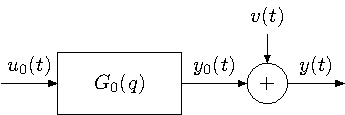
\includegraphics{\thisDir/figs/tikz0.pdf}
\caption{SISO LTI discrete-time system in an output error setup.}
\label{lpmtdrep}
\end{figure}

Numerous parametric identification techniques are devoted to the development of parametric plants $G(q,\theta)$ and parametric noise models  $H(q,\theta)$, where  $\theta$ is the model parameters vector  \citep{Ljung1999,Soderstrom1989}.

In this section, however, a nonparametric technique is developed, %the identification problem is
formulated in the frequency domain, consistent with \citep{Pintelon2012,Mahata2006}. The following  choices are made:

\begin{itemize}

\item

The work in this section is for discrete-time systems. Denote the $k^{th}$ discretized frequency as $\Omega_k$ = $e^{-j2{\pi}kf_s/N}$, with $f_s$ the sample frequency and $N$ the total number of sample points.
\item

Describe the parametric plant model  $G(q,\theta)$ by the nonparametric \gls{FRF} counterpart  $G(\Omega_k)$  at the $k^{th}$ frequency.
\item

Describe  the parametric noise model $H(q,\theta)$ (associated with the output noise source $v(t)$) by a nonparametric noise variance contribution $\sigma^2_v(\Omega_k)$ at the $k^{th}$ frequency.

\end{itemize}

The rest of the section is structured as follows. \secref{se:theoryLPMandWindowing} covers the theory on the \gls{LPM} and windowing for an \gls{OE} setup.
\secref{se:smoothingFRFestimate} discusses the novel smoothing method.



Ultimately, in \secref{se:simResults}, simulation results of the following FRF estimates and their corresponding variances are compared: (i) the smooth \gls{LPM} estimate $\hat{G}_\text{sm-poly}(\Omega_k)$, (ii) the \gls{LPM} estimate $\hat{G}_\text{poly}(\Omega_k)$.

These FRF estimates are also compared with the true \gls{LTI} system ${G}_0(\Omega_k)$.
Discussion of the simulation results is then followed by a conclusion in \secref{se:conclusion}.

\subsection{Theory on the LPM and Windowing: \glsentrytext{OE} Setup}
\label{se:theoryLPMandWindowing}

Details of the theory pertaining to this section may be found in \citep{Schoukens2009LPM}, basic aspects of which are presented below.


\subsubsection{Spectral Nonparametric Model and Assumptions}

Using convolution, the noiseless output signal in \figref{lpmtdrep} is $y_0(t) = g_0(t)*u_0(t)$, where the signals are sampled at $t = 0, 1, 2,...,N-1$ and the excitation signal $u_0(t)$ is random noise. As shown in \citep{Pintelon2012} and \citep{Pintelon1997} the \gls{DFT} spectra of the sampled signals at the frequency $\Omega_k$ are related as follows:
\begin{equation}\label{lpmleak}
Y_0(k)=G_0(\Omega_k)U_0(k)+T_G(\Omega_k)
\end{equation}
where $U_0(k)$ is the \gls{DFT} spectrum of the random noise excitation,  $G_0(\Omega_k)$ is the transfer function and $T_G(\Omega_k)$ is the transients leakage term.
In this section, the \gls{DFT} of a signal $x(t)$ is defined explicitly as  \citep{Oppenheim1983}

\begin{equation}\label{eq:defDFT}
X(\Omega_k) = \frac{1}{\sqrt{N}}\sum_{t=0}^{N-1}x(t)e^{-\frac{j2\pi kt}{N}}
\end{equation}


The following assumptions are consistent with \citep{Schoukens2009LPM} for an OE setup (\figref{lpmtdrep}):
\begin{assumption}
The \gls{SISO} system $G_0$ and  the transients leakage spectrum $T_G$ are both smooth functions of the frequency.
\end{assumption}



\begin{assumption}

The spectrum of the  input signal $U_0$ is not a smooth function of the frequency, but a rough function, for example $U_0(k+1) - U_0(k)$ should not vanish to zero. %i.e. $U_0(k+1) - U_0(k) \neq 0$.
\TODO{assumption is not complete! some expectation is missing!}
\end{assumption}

In other words, for the excitation signal to be rough: the magnitude of the spectral difference $|U_0(k+1) - U_0(k)|$ must have a probability of 1 (unity) for it to remain in the same order of magnitude as $|U_0(k)|$, irrespective of the record length $N\rightarrow\infty$ and the corresponding  frequency resolution $f_0\rightarrow{0}$.


\begin{assumption}
The measured output signal is $y(t) = y_0(t) + v(t)$ with the exact input signal $u_0(t)$ known.
\end{assumption}


\begin{assumption}
The filtered white noise $v(t) = H_0(q)e(t)$ is the disturbing noise source at the output.
\end{assumption}


\subsubsection{The Hanning Window and the \glsentrytext{LPM}}\label{se:LPMFRFest}%\label{se:FRFhanningLPM}
\paragraph{Windowing}
The effect of windowing may be  exemplified by use of the Hanning window, which is very popular.
In a nutshell, the Hanning window is effective in reducing  the leakage errors, but  with a trade off of increased interpolation errors. %This is because the term $G_0(\Omega_k)U_0(k)$ in equation \eqref{eq:lpm:TD} is not smooth and $G_0(\Omega_k)$ varies with the frequency.
Pertinent details of the Hanning window are discussed in \citep{Schoukens2006LPM,Antoni2007FRF,Schoukens2009LPM,Wellstead1981} and \citep{Harris1978}.

The anomalies due to interpolation errors, associated with windowing, can easily be mitigated or circumvented by use of the \gls{LPM}. As shown in \citep{Pintelon2012}, the leakage errors are reduced from  $\mathcal{O}({N}^{-1})$, for Hanning windowing, to $\mathcal{O}({N}^{-3})$ or better, for the \gls{LPM}.


\paragraph{Formulation of the Linear LS LPM}
The \gls{LPM} is formulated as a nonparametric local-linear-least-squares (LS) estimate using the full data record of length $N$ as outlined below \citep{Schoukens2009LPM}.
\citet[Section 7.2.2]{Pintelon2012} gives the general formulation of the \gls{LPM} for \gls{MIMO} systems.
The formulation in this section is a summary for a \gls{SISO} system.

The \gls{DFT} spectra at the output of the \gls{SISO} system in \figref{lpmtdrep} are derived from equations \eqref{eq:lpm:TD} and \eqref{lpmleak}, \emph{viz}:
\begin{equation}\label{lpm1spectra}
Y(k)=G_0(\Omega_k)U_0(k)+T(\Omega_k)+V_0(k)
\end{equation}
where $V_0(k) = H_0(\Omega_k)E(k)$ is a noise term, and $T(\Omega_k)$ is the leakage term. The latter is the sum of the system and the noise leakage terms, i.e. $T(\Omega_k) = T_G(\Omega_k) + T_H(\Omega_k)$.

The smooth characteristics of $G_0(\Omega_k)$ and $T(\Omega_k)$ allow for the use of the Taylor series representations at the frequency lines $k+r$ in a frequency domain window of width $2n+1$, with a remainder $\bigO{\left(\frac{r}{N}\right)^{R+1}}$ of the first order Taylor series expansion \citep{Schoukens2009LPM}, \emph{viz}:
\begin{align}\label{lpmGTaylorS}
G_0(\Omega_{k+r})&=G_0(\Omega_k)+\sum_{p=1}^{R}g_p(k)r^p+
\bigO{\left(\frac{r}{N}\right)^{R+1}},
\\
\label{lpmTTaylorS}
T(\Omega_{k+r})&=T(\Omega_k)+\sum_{p=1}^{R}t_p(k)r^p+N^{-1/2}
\bigO{  \left(\frac{r}{N}\right)^{R+1}  }
,
\\
\text{where}&\ r\in\mathbb{W}_n,\quad \mathbb{W}_n = \{-n,-n+1,\dots,n\}
\end{align}

The choice of the tunable parameters $n$ and $R$ is discussed later on.

Neglecting the remainder, the Taylor series approximation of \eqref{lpm1spectra} can be written in a matrix vector form, \emph{viz}:
\begin{equation}\label{lpmGTMatrix}
Y(k+r)\approx{K(k, r)\theta(k)+V_0(k+r)}
\end{equation}
where $\theta(k)\in\mathbb{C}^{2R+2}$ is the column vector of the  parameters ($G_0(\Omega_k)$, $T(\Omega_k)$, $g_p$, $t_p$, and $p = 1, 2, ...., R$) and $K(k, r)$ is the row vector of their respective coefficients:
\begin{align}
K(k,r) = &\left[
\begin{matrix}
U_0(k+r) & U_0(k+r)r & \dots
\end{matrix}
\right.
\\
&\quad\left.\begin{matrix}U_0(k+r)r^R & 1& r&\dots&r^R\end{matrix}\right]\nonumber
\end{align}


Equation \eqref{lpmGTMatrix} can be written in the more compact (stacked vectors) form:
\begin{equation}\label{lpmGTMatrixStack}
Y_n(k)\approx K_n(k)\theta(k)+V_n(k)
\end{equation}
where $Y_n(k), V_n(k)\in\mathbb{C}^{2n+1}$, and $K_n(k)\in\mathbb{C}^{(2n+1)\times(2R+2)}$ are the stacked values of $Y(k+r)$, $K(k,r)$, and $V_0(k+r)$, respectively, for $r\in\mathbb{W}_n$.
The estimates of the parameters $\theta(k)$ are obtained as the minimizers of the least squares problem, \emph{viz}:
\begin{align}\label{eq:LSsolutionLPM}
\hat\theta(k) = \argmin_{\theta(k)} \left\|Y_n(k) - K_n(k)\theta(k)\right\|_2^2
\end{align}

The formulation of equation \eqref{eq:LSsolutionLPM} must take into account the fact that  a full rank of $K_n$ requires $n \geq R + 1$. The choice $n = R + 1$ results in the highest variance on the estimate, but with the smallest interpolation error \citep{Schoukens2009LPM}.


The values $R = 2$, and $n=R+1=3$ will be used in the \gls{LPM}.

When substituted into equations \eqref{lpmGTaylorS} and \eqref{lpmGTMatrix},  these yield the following quadratic local polynomials of $G_0$ and $T$ around a central frequency $\Omega_{k}$:
\begin{align}
G_0(\Omega_{k+r})
  &\approx 
  G_0(\Omega_k)+g_1r+g_2r^2
  \label{eq:lpm:expansionG:quadratic}
\\
  T(\Omega_{k+r})
    &\approx 
    T(\Omega_k)+t_1r+t_2r^2
    \label{eq:lpm:expansionT:quadratic}
\end{align}
with ($r\in\mathbb{W}_3$) and the vector of parameters:
\begin{equation}\label{lpmThetaEst}
\theta^\top(k)=\left[G_0(\Omega_k) \ g_1 \ g_2\  T_G(k)\  t_1 \ t_2\right]
\end{equation}
The \gls{LPM} estimate of the \gls{FRF} is the first element of the estimate $\hat\theta(k)$, obtained from \eqref{eq:LSsolutionLPM}, \emph{viz}:
\begin{equation}
\hat{G}_\text{poly}(\Omega_k) = \hat\theta_1(k)
\end{equation}


The estimation of $\hat{G}_\text{poly}(\Omega_k)$ at a single frequency $\Omega_k = 0.586\unit{Hz}$ is illustrated in \figref{LPM_Schematic_EG}.% centered at $k$, where $r = 0$.
\begin{figure}[htb] %  figure placement: here, top, bottom, or page
   \centering
   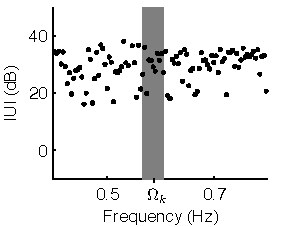
\includegraphics[scale=0.92]{\thisDir/figs/spectUOmegak}
   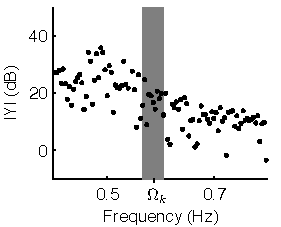
\includegraphics[scale=0.92]{\thisDir/figs/spectYOmegak}
   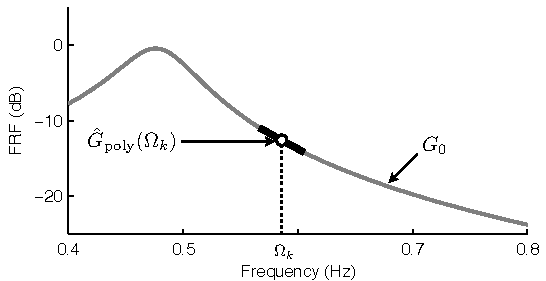
\includegraphics{\thisDir/figs/LPMfigOmegak}
   \caption{Illustration of the \gls{LPM}. Top figures: input spectrum (left) and output spectrum (right). A small band is selected (gray area, top figure), in which $\hat G_\mathrm{poly}(\Omega_{k+r})$ is estimated (black thick line, bottom figure) as a local polynomial. Only its central value $\hat G_\mathrm{poly}(\Omega_k)$ (white circle) is retained. This procedure is repeated for all $\Omega_k$.}
   \label{LPM_Schematic_EG}
\end{figure}
This procedure is repeated at each central frequency $\Omega_k$ for  $k\in \Set{1,\dots,N/2}$ (i.e. the entire frequency band, including Nyquist, but excluding \gls{DC}, and regularizing at the boundaries). This completes the \gls{LPM}, yielding an intrinsic averaging of the spectra of the estimated \gls{FRF}, $\hat{G}_\text{poly}(\Omega_k)$.

\section{Smoothing the \gls{FRF} estimate}\label{se:smoothingFRFestimate}
The method for smoothing (improving) the \gls{LPM} estimate of the frequency response function  is presented in this section together with pertinent assumptions. After obtaining the \gls{LPM} estimate of the \gls{FRF} (denoted as $\hat{G}_{\mathrm{poly}}(\Omega_k)$) from \secref{se:LPMFRFest}, the smoothing method is decomposed into the following procedures, which will be elaborated on later:
\begin{enumerate}
\item The impulse response $\hat g_\mathrm{poly}(t)$  is computed from the \gls{IDFT} of $\hat{G}_{\mathrm{poly}}(\Omega_k)$.

\item
Assuming that the impulse response decays exponentially in time, the noise is bound to predominate after a certain time interval.

\item
An accurate estimate of the \gls{DC} value of the \gls{FRF} is computed by inspecting the average value of the tail of the estimated impulse response.

\item
A truncation is effected at the point beyond which the data record (impulse response) is buried in noise.

This action results in smoothing the \gls{LPM} estimate of the \gls{FRF}.
An exponential fitting method is introduced to determine the truncation point.
\end{enumerate}

These procedures require that the following assumptions are satisfied.

\begin{assumption}
The estimate $\hat G_\mathrm{poly}(\Omega_k)$ is available at all frequencies $\Omega_k$ for $k\in\{1,2,\dots,N/2\}$.
\end{assumption}

This assumption ensures that the impulse response corresponding to the \gls{FRF} can be computed (up to its mean value). It requires that the input signal excites the whole unit circle. This is satisfied, for instance, by using white noise as an excitation signal.


\begin{assumption}\label{ass:imprespdecay}
The impulse response $g(t)$ decays exponentially over time, i.e. $\exists A \in \PositiveRealNumbers, \exists a \in \NegativeRealNumbers \without \Set{0}, \forall t \in \PositiveRealNumbers: \abs{g(t)} \leq A \exp(- a t)$.
\end{assumption}

\begin{assumption}\label{ass:decay90perctime}
Within $90\%$ of the measurement window, the impulse response decays
 to a level that is indistinguishable from the noise.
\end{assumption}

Note that Assumptions \ref{ass:imprespdecay} and \ref{ass:decay90perctime} exclude the possibility of considering a system that is a pure integrator.

\subsubsection{Obtaining the Impulse Response Function}

The estimated impulse response function  $\hat g_{\mathrm{poly}\setminus \mathrm{DC
}}(t)$ is obtained explicitly via the \gls{IDFT} of the \gls{LPM}-estimate $\hat G_\mathrm{poly}(\Omega_k)$ of the \gls{FRF} in accordance with equation \eqref{eq:defDFT}, \emph{viz}:

\begin{align}\label{eq:impRespiDFT}
\hat g_{\mathrm{poly}\setminus \mathrm{DC
}}(t) &= \frac{1}{\sqrt{N}}\sum_{k=1}^{N-1}\hat G_\mathrm{poly}(\Omega_k)e^{\frac{j2\pi kt}{N}}
\end{align}
where the estimated \gls{FRF} in the frequency band between  the Nyquist and the sample frequencies is obtained as follows:

\begin{align}
\hat G_\mathrm{poly}(\Omega_{N-k}) = \overline{\hat G_\mathrm{poly}(\Omega_k)},\ \text{for}\ k=1,\dots,N/2
\end{align}
(with $\conj{\hat G_\mathrm{poly}}$ the complex conjugate of $\hat G_\mathrm{poly}$) to ensure $\hat g_\mathrm{poly}(t)$ to be real.

\TODO{fix reference Section II}
Smoothing of the estimated \gls{FRF} requires the correct estimate of the impulse response. Unfortunately, the \gls{LPM} presented in \secref{se:theoryLPMandWindowing} and in \citep{Schoukens2009LPM} does not estimate the \gls{FRF}  at the frequency $\Omega_0$ (i.e. \gls{DC} value of the \gls{FRF}), hence the subscript $\setminus\mathrm{DC}$ in equation \eqref{eq:impRespiDFT}. Consequently, the mean value of the corresponding estimated impulse response given in equation \eqref{eq:impRespiDFT} is not correct. 
This limitation is lifted by developing a simple estimator of the mean value, presented below.

\subsubsection{Estimating the \glsentrytext{DC} Value of the \glsentrytext{FRF}}\label{se:DCvalueEst}
The correct mean value of the impulse response accounts for (i.e. estimates) the \gls{DC} value of the \gls{FRF}. A time-domain method is proposed for estimating the mean value of the impulse response in equation \eqref{eq:impRespiDFT}. %The first is a frequency-domain technique and the second is a time-domain technique.

According to Assumption~\ref{ass:imprespdecay}, the true impulse response tends to zero asymptotically; and by Assumption~\ref{ass:decay90perctime}, the last $10\%$ of the estimated impulse response is noise, plus a constant value due to an inaccuracy in the average value of the impulse response. The correct estimate of the mean value is obtained by shifting the whole signal such that the last $10\%$ of the impulse response is centered around 0.
To this end, the following procedure is executed:


\begin{enumerate}
\item Compute the mean value $m_{g10}$ of the last 10\% of the impulse response $\hat g_{\mathrm{poly}\setminus \mathrm{DC
}}(t)$, estimated by the \gls{LPM}, as %$\hat g_\mathrm{poly}(t)$ as
\begin{align}
m_{g10} = \frac{1}{\lceil0.1N - 1\rceil}\sum_{t=\lfloor0.9N\rfloor}^{N-1}\hat g_{\mathrm{poly}\setminus \mathrm{DC
}}(t)
\end{align}

\item Next, subtract the computed mean value $m_{g10}$ from $\hat g_{\mathrm{poly}\setminus \mathrm{DC
}}(t)$ to obtain the improved impulse response $\hat g_\mathrm{poly}(t)$, \emph{viz}:


\begin{align}
\hat g_\mathrm{poly}(t) = \hat g_{\mathrm{poly}\setminus \mathrm{DC
}}(t) - m_{g10},\ \text{for}\ t=0,1,\dots,N-1
\end{align}


\end{enumerate}

\subsection{Truncation of the Impulse Response Via Exponential Fitting}\label{se:truncImpulseResp}

The \gls{FRF} estimate is smoothed by truncating the estimated impulse response function. 
The truncation is applied at the time index beyond which the signal is indistinguishable from the noise.

This is done via the fit of an exponential function on the maxima of the impulse response, implemented as follows.

\begin{enumerate}
\item Obtain the estimate of the impulse response $\hat g_\mathrm{poly}(t)$ from the \gls{LPM}, corrected for its \gls{DC} value as discussed in \secref{se:DCvalueEst}. Henceforth, $\hat g_\mathrm{poly}(t)$ will simply be denoted as $\hat g(t)$. %In the remainder of this procedure description $\hat g_\mathrm{poly}(t)$ will be simply denoted $\hat g(t)$.

\item Obtain an estimate $\hat \sigma_\mathrm{n}$ of the standard deviation of the noise from the last 10\% of the data, \emph{viz}:

\begin{align}
\hat \sigma^2_\mathrm{n}=\frac{1}{\lceil0.1N - 1\rceil}\sum_{t=\lfloor0.9N\rfloor}^{N-1}\hat g^2(t).
\end{align}
This is valid, as per Assumption \ref{ass:decay90perctime}.

%This assumes that the impulse response of the system is not longer than 90\% of the length of the measured time interval.

\item Obtain $\mathbb{T}_\mathrm{HSNR}$ as the set of time instants where $\hat g(t)$ is significantly above the standard deviation of the noise. Only samples with absolute values of at least $5\hat\sigma_\mathrm{n}$ are retained: %Only samples with an absolute value of at least $5\hat\sigma_\mathrm{n}$ have been retained:
\begin{align}
\mathbb{T}_\mathrm{HSNR} = \left\{
t:|\hat g(t)|\geqslant 5\hat\sigma_\mathrm{n}
\right\}.
\end{align}
(Subscript HSNR stands for High \gls{SNR}.)

%This choice leaves a probability of $6\times10^{-7}$ of retaining a pure noise sample, in the case of Gaussian noise.

\item Find the set $\mathbb{T}_\mathrm{max}$ of indices corresponding to monotonically decreasing maxima of the impulse response:
\begin{align}\label{eq:TmaxDef}
\mathbb{T}_\mathrm{max} = \left\{
t: \left| \hat g(t)\right|>
\left|\hat g(t')\right|,
t < t' < N \land t'\in\mathbb{T}_\mathrm{HSNR}
\right\},
\end{align}

\item Fit an exponential function $Ae^{at}$ approximating $\hat g(t)$, in $t_\mathrm{max}\in\mathbb{T}_\mathrm{max}$. 
This is done by solving the following expression

\begin{align}\label{eq:expFit}
\ln \left|\hat g(t)\right|\approx \ln A+at,\ \mathrm{with}\ t\in\mathbb{T}_\mathrm{max},
\end{align}
for $\ln A$ and $a$ in a least squares sense.
This is a quadratic problem in the parameters and, thus, amount to a convex optimization problem that can be solved directly.
Since  $\ln \left|\hat g(t)\right|$ decreases for an increasing $t$ in $\mathbb{T}_\mathrm{max}$ (by construction in equation \eqref{eq:TmaxDef}), the estimated $a$ from equation \eqref{eq:expFit} is always negative.

\item
Determine the first time-instant $t_\mathrm{trunc}$ at which the estimated exponential gets significantly below the noise floor, \emph{viz}:
\begin{align}\label{eq:truncTimeExpFit}
t_\mathrm{trunc} = \min \left\{t:Ae^{at} < \gamma\hat\sigma_\mathrm{n}\right\}
\end{align}
where the parameter $\gamma$ can be tuned such that an appropriate trade-off between the decreased variance and the increased bias on the estimated smoothed FRF is found. This is discussed below. %(see the discussion below).
% The value of $\gamma$ to be used depends on the system. %$\gamma = 0.1$ was found to be a good rule of thumb.

\item
 Truncate the estimated impulse response for $t \geqslant t_\mathrm{trunc}$.

\end{enumerate}

\begin{figure}[tbh] %top bottom here
\centering

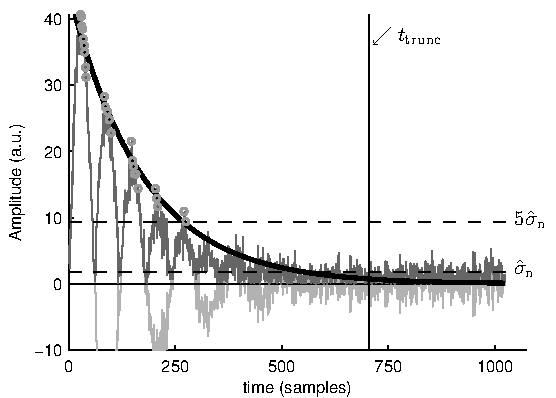
\includegraphics[scale=0.9]{\thisDir/figs/expFitest}
\caption{Truncation of the impulse response via the fit of  an exponential. The light gray line is the noisy impulse response, and the dark gray one is its absolute value. Gray circles: monotonously decreasing maxima, greater than $5\hat\sigma$, as per \eqref{eq:TmaxDef}. Black thick line: estimated exponential function \eqref{eq:expFit}.}
\label{FRF_truncate_expfitter}
\end{figure}

As an illustration, this procedure was applied to the noisy impulse response of the system described by the following difference equation:

\begin{equation}
y_0(t) = 2.583y_0(t - 1) -2.176y_0(t - 2)+0.592y_0(t-3) + u(t)
\end{equation}

The measured signal was disturbed by random white noise, $y(t) = y_0(t) + e(t)$, such that the \gls{SNR} was $14.2\unit{dB}$.
The result is depicted in \figref{FRF_truncate_expfitter}. An exponential function (black thick line) is fitted on the maxima (gray circles) of the absolute value of a noisy impulse response (dark gray line). The truncation time (black vertical line) $t_\mathrm{trunc}$ was selected as the time instant at which the fitted exponential fell below $0.4\hat\sigma_n$ (i.e. $\gamma = 0.4$ in equation \eqref{eq:truncTimeExpFit}).

\paragraph*{Considerations on the choice of $\gamma$}

\begin{itemize}
\item The tuning parameter $\gamma$ is application- and system-dependent.  A higher value lowers the variance of the estimated \gls{FRF}, but increases its bias, and vice versa.

\item
The bias error is highest in the vicinity of (sharp) resonance peaks. If the latter is to be estimated with a high accuracy, a value $\gamma \ll 1$ must be used. %If the latter must be estimated with a high accuracy, a value $\gamma \ll 1$ must be preferred.

\item If one is interested in obtaining a smooth initial estimate of the \gls{FRF}, a (small) bias error is acceptable, and choosing $\gamma \approx 1$ was found to be a good rule of thumb.
\end{itemize}

\subsection{Simulation Results}\label{se:simResults}

\figref{figLPMvsTrunc} and \figref{fig:pdfAndRMSeVStruncTime} compare the \gls{LPM} with and without truncation of the impulse response.
They were obtained from simulations on  the system described by the following simulation equations, which are relevant to the \gls{LPM} outlined in \secref{se:LPMFRFest}:
\begin{subequations}
\label{eq:systemSimulations}
\begin{align}
y_0(t)  &= 1.5371y_0(t-1)    -0.9025y_0(t-2) + u(t)
\\
y(t) &= y_0(t) + e(t),
\end{align}
\end{subequations}
where $e(t)$ is a white noise sequence, such that the \gls{SNR} of the output signal is $18.3\unit{dB}$.


\begin{figure}[tbh] %top bottom here
\centering


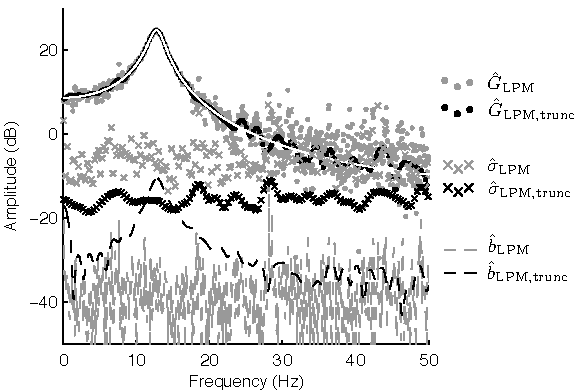
\includegraphics[scale=0.9]{\thisDir/figs/figLPMvsTruncWlegend}

\caption{Comparison of the \gls{LPM} and Truncated \gls{LPM} estimates of the \gls{FRF} for an \gls{SNR} of $18.3\unit{dB}$. The gray plots pertain to the \gls{LPM} estimate without truncation, the black ones to the \gls{LPM} with truncation (trunc). Dots: \gls{FRF} estimates $\hat{G}$. Crosses: sample standard deviations $\hat{\sigma}$. Dashed lines: bias $\hat{b}$. White line: the true system $G_0$.}
\label{figLPMvsTrunc}
\end{figure}





In \figref{figLPMvsTrunc} one observes the following:
\begin{itemize}
\item
a decrease of the variance on the truncated estimate of about $10 \unit{dB}$,  i.e. a decrease of the black crosses, compared to the gray ones, is observed. %i.e. a decrease of the black crosses w.r.t.~the gray ones is observed.

\item
the error on the truncated \gls{LPM} estimate is strongly correlated over the frequency. This must be taken into account when formulating a maximum likelihood parametric estimator of the system.

\item
an increase of the bias of the truncated estimate, especially in the vicinity of the resonance frequency. Still, this bias lies below the variance of the non-truncated estimate. As such, for a single experiment, the increase in bias still yields a better estimate when truncation is invoked.

This bias depends on the time instant at which the truncation is performed, as discussed below.

\end{itemize}

\begin{figure}[htb] %  figure placement: here, top, bottom, or page
   \centering



	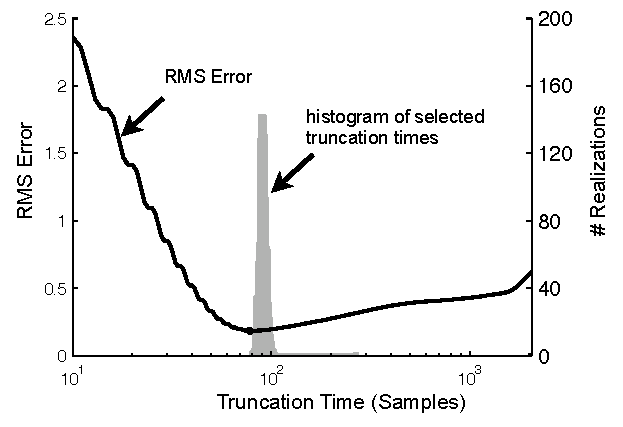
\includegraphics{\thisDir/figs/HistogramExpFitting.pdf}
 \caption{Black full line (left hand side y-axis (ordinate)): total \gls{RMS} error as a function of the truncation time (the single black dot is the minimum of the \gls{RMS}). Gray histogram (right hand side y-axis (ordinate)): selected truncation times for 1000 noise realizations by the exponential fitting methods.}



   \label{fig:pdfAndRMSeVStruncTime}
\end{figure}

In \figref{fig:pdfAndRMSeVStruncTime}, the black graph is the \gls{RMS} error of the estimated \gls{FRF} (without the \gls{DC} value) as a function of the time $t_\mathrm{trunc}$ at which the impulse response is truncated. Its minimum is indicated by a black dot, to the left of which a steep increase is observed. This is due to a bias error. To the right hand side of the minimum, the \gls{RMS} error increases very gradually, due to an increase of the noise variance.

A good practice would be to truncate the impulse response at the minimizer (black dot) of the \gls{RMS} error. However, it should be noted that this minimizer is unknown in practice, because it would require
the true \gls{FRF}.

The truncation time is determined from the data as described in \secref{se:truncImpulseResp}. This was done on $1000$ realizations of the noise, and depicted in \figref{fig:pdfAndRMSeVStruncTime} by the histogram.
Clearly, the method for selecting the truncation time $t_{\mathrm{trunc}}$ has a good overall performance, based on the mode of its distribution. A closely grouped set of values for $t_{\mathrm{trunc}}$ is obtained around the $90^{\text{th}}$ sample, without significant outliers.


From the plot, we can conclude that the \gls{RMSE} increases rapidly when $t_{\mathrm{trunc}}$ is smaller than the optimal.
On the other hand, selection of a value of $t_{\mathrm{trunc}}$ that is too large, is not nearly as detrimental to the modeling error.
The graph also shows that the \gls{RMSE} of the model can be decreased from $0.62$ (without truncation) to $0.18$ when the optimal truncation is applied. Also, one observes a low sensitivity of the \gls{RMSE} w.r.t.~$t_\mathrm{trunc}$, when truncating at times beyond that optimum. Therefore, a somewhat conservative truncation method is still likely to yield a close to optimal result.

\subsection{Conclusion}\label{se:conclusion}

The section introduced a novel time domain method to smooth the \gls{LPM}-estimate of an \gls{FRF}. It consisted of, after obtaining the \gls{FRF} from the \gls{LPM}, computing the associated estimated impulse response via the \gls{IDFT}.
Then, it was determined statistically at which time index the impulse response had decayed below the noise floor, yielding a point beyond which the response may be set to zero.

The results clearly indicate that the truncation technique lowers the impact of the noise on the estimate of the \gls{FRF}, resulting in a decreased variance. A bias-variance trade-off is possible by tuning the time beyond which the impulse response is indistinguishable from the noise.


  \section{Conclusion}
  \label{sec:conclusion}

  \begin{itemize}
    \item LRM: extension to LRIC
    \item LRM: derivation of bias
    \item LRM vs LPM: at which settings is LRM better than LPM
    \item LRIC: much slower, performance is somewhat better, but at the cost of a lot of computational power and much harder model selection
    \item practical advice: use LRM rather than LPM unless in very noisy conditions (10 dB), only use LRIC as last resort
  \end{itemize}


% \begin{subappendices}
  \section{Proof of the \glsentrytext{LOOCV} statistic for linear models}

  We follow an approach similar to \citet{Hyndman2014LOOCV} and \citet[Section 12.3.2]{Seber2003} to prove that for a linear model, one can easily compute the \gls{PRESS}/\gls{LOOCV} statistic by means of the so-called `hat-diagonals', the diagonal entries of the hat matrix $H$.
  This is relevant, e.g. for local linear models used in the \gls{LRM} and hence also the \gls{LPM}.

  We consider the linear model
  \begin{equation}
    Z = K \theta + V
  \end{equation}
  with $Z \in \ComplexMatrix{N\times1}$, $\theta \in \ComplexMatrix{\nth \times 1}$, $K \in \ComplexMatrix{N \times \nth}$.
$V \in \ComplexMatrix{N \times 1}$ is a \gls{iid} complex gaussian random variable.
The least-squares solution of such a linear model is:
\begin{equation}
  \hat{\theta} = \left(K^{\HT} K \right)^{-1} K^{\HT} Z = \pinv{K} Z
\end{equation}
such that the estimated output $\hat{Z}$ is given by
\begin{equation}
  \hat{Z} = K \pinv{K} Z = H Z
\end{equation}
where $H$ is the so-called `hat matrix' that projects the measurements $Z$ onto the estimates $\hat{Z}$.

The \gls{PRESS} statistic used in \gls{LOOCV} is defined as~\citep[Chapter 12]{Seber2003}
\begin{equation}
  \PRESS \isdef 
    \frac{1}{N} 
      \sum_{i=1}^{N}
      \abs{
        Z_i - \ignoring{i}{\hat{Z}}
      }^2
\end{equation}
where $\hat{Z}_i$ is the $i^{\text{th}}$ row of $\hat{Z}$ and $\ignoring{i}{\hat{Z}}$ denotes the estimated $\hat{Z}_i$ when the $i^{\text{th}}$ data point (i.e. row) is removed from the estimation problem.
For linear models, this is equivalent to
\begin{equation}
  \PRESS_{\mathrm{linear}} = 
     \frac{1}{N}
     \sum_{i=1}^{N}
     \abs{
       \frac{Z_i - \hat{Z}_i}
                {1 - H_{ii}}
     }^2
     \text{.}
\end{equation}
Note that in this last expression, no terms $\ignoring{i}{\hat{Z}}$ occur, such that the statistic can be computed without having to compute $N$ additional linear models.
In this appendix, we prove that these last two expressions are equivalent for linear models.

\paragraph{Proof}
\TODO{proof}
Denote the design matrix $\ignoring{i}{K}$ to be the design matrix $K$ where the $i^{\text{th}}$ row has been removed:
\begin{equation}
  \ignoring{i}{K}
  \isdef
  \begin{bmatrix}
    K_{1,1} & K_{1,2} & \cdots & K_{1,\nth}\\
   && \vdots\\
    K_{i-1,1} & K_{i-1,1} & \cdots & K_{i-1,\nth}\\
    K_{i+1,1} & K_{i+1,1} & \cdots & K_{i+1,\nth}\\
    && \vdots\\
    K_{N,1} & K_{N,2} & \cdots & K_{N,\nth}\\
  \end{bmatrix}
\end{equation}

\begin{lemma}[Matrix Inversion Lemma]\label{lem:matrix-inversion-lemma}
The Woodbury formula, states that
\begin{equation*}
\left(A+UCV \right)^{-1} 
= 
A^{-1} - A^{-1} U \left(C^{-1}+VA^{-1}U \right)^{-1} VA^{-1}
\end{equation*}
when the dimensions of the matrices allow for the multiplications~\citep[Section 3.2.2]{matrixcookbook}.
\end{lemma}

\TODO{evt. Seber2003/ChristensenXXXX: QR decomposition to compute $H$}


\end{subappendices}

